\chapter{Introducción, alcance del proyecto.}

Este proyecto desarrolla una versión del juego clásico "Simon Dice," utilizando un enfoque innovador basado en reconocimiento visual y procesamiento de imágenes. La propuesta combina elementos de calibración de cámaras, detección de patrones y análisis de figuras geométricas para ofrecer una experiencia interactiva y dinámica.

\section{Descripción General}
El sistema utiliza la cámara del dispositivo para capturar y analizar las acciones del usuario en tiempo real. A lo largo del juego, se generan secuencias aleatorias de figuras geométricas para cada nivel. El jugador debe reproducir estas secuencias utilizando gestos, los cuales son detectados y evaluados por el sistema.

\section{Principales Componentes del Proyecto:}
\subsection{Calibración de Cámara:}
Se lleva a cabo un proceso inicial de calibración para garantizar una captura precisa y sin distorsión de las imágenes. Esto permite mejorar la fiabilidad de los resultados en etapas posteriores de detección. Se han utilizado patrones de tablero de ajedrez para calcular las esquinas y con ello poder obtener los parámetros intrínsecos de la cámara. Podemos observar en la figura el RMSE a medida que se añaden imagenes a la calibración.

\begin{figure}[H]
    \centering
    \begin{minipage}{0.45\textwidth} 
        \centering
        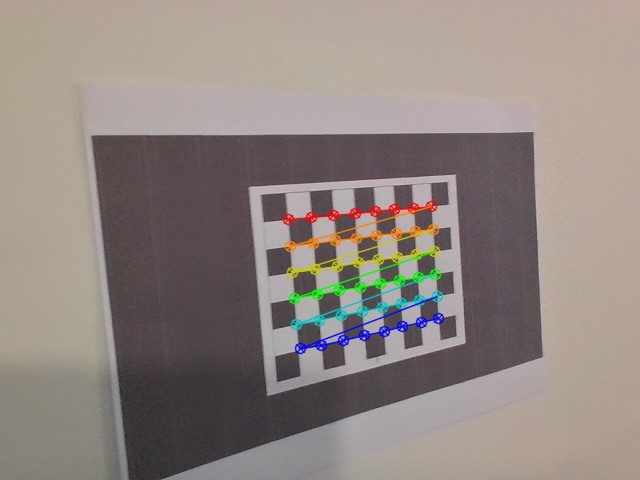
\includegraphics[width=\linewidth]{CAPS/CAP1.jpg}
        \caption{Imagen de calibración con corners.}
        \label{fig:imagen1}
    \end{minipage}\hfill
    \begin{minipage}{0.45\textwidth} 
        \centering
        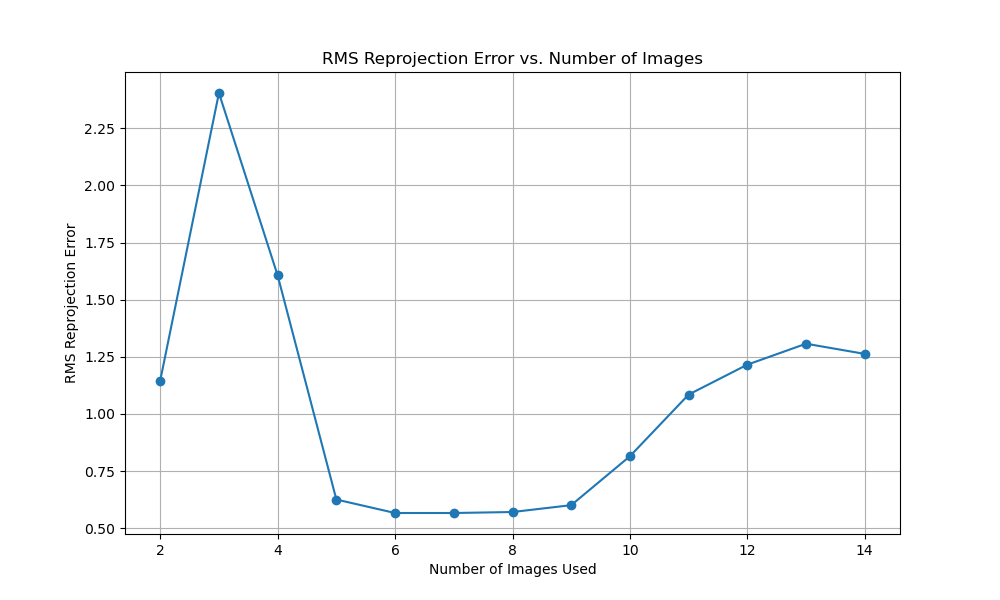
\includegraphics[width=\linewidth]{CAPS/CAP2.png}
        \caption{Root Mean Square Error en función del número de imágenes.}
        \label{fig:imagen2}
    \end{minipage}
\end{figure}


\subsection{Detección y Seguimiento de Patrones:}
Mediante algoritmos avanzados de visión por ordenador, como el uso de técnicas basadas en MediaPipe, se identifican y rastrean los movimientos de las manos y otros gestos del jugador.

\subsection{Reconocimiento de Formas Geométricas:}
Las trayectorias generadas por los movimientos del usuario son procesadas para identificar figuras geométricas. Esto incluye la creación de máscaras y la detección de contornos, asegurando que el sistema reconozca con precisión las formas reproducidas.

\subsection{Validación de Secuencias:}
El sistema compara las figuras detectadas con las secuencias aleatorias generadas previamente, validando si el jugador ha completado correctamente el nivel.

\subsection{Progresión por Niveles:}
A medida que el usuario avanza, las secuencias se vuelven más complejas, aumentando así la dificultad del juego.
